\documentclass[11pt,a4paper]{article}

\usepackage[utf8]{inputenc}
\usepackage[T1]{fontenc}
\usepackage[spanish,es-noindentfirst]{babel}
\usepackage[margin=2.5cm]{geometry}
\usepackage{graphicx}
\usepackage{booktabs}
\usepackage{longtable}
\usepackage{array}
\usepackage{xcolor}
\usepackage{hyperref}
\usepackage{caption}
\usepackage{amsmath}
\usepackage{amssymb}
\usepackage{float}
\usepackage{microtype}
\usepackage{seqsplit}
\emergencystretch=3em
\tolerance=1200
\newcommand{\nb}[1]{\texttt{notebooks/}\allowbreak\texttt{#1}}
\usepackage{enumitem}
\usepackage{tikz}
\usetikzlibrary{arrows.meta,positioning,shapes.geometric}
\usepackage{fancyhdr}
\usepackage{titlesec}

\hypersetup{colorlinks=true, linkcolor=blue!50!black, citecolor=blue!50!black, urlcolor=blue!50!black}
\captionsetup{font=small, labelfont=bf}
\titleformat{\section}{\normalfont\Large\bfseries}{\thesection}{1em}{}
\titleformat{\subsection}{\normalfont\large\bfseries}{\thesubsection}{1em}{}

\newcommand{\ok}{\textcolor{green!50!black}{\checkmark}}
\newcommand{\fail}{\textcolor{red}{$\times$}}
\newcommand{\supuesto}[1]{\textit{[Supuesto: #1]}}

\pagestyle{fancy}
\fancyhf{}
\fancyhead[L]{\small Sistema Adaptativo de Predicción de Reingreso Hospitalario}
\fancyhead[R]{\small UTEC · Planificación y Toma de Decisiones en IA}
\fancyfoot[C]{\thepage}

\title{\textbf{Sistema Inteligente Adaptativo para la Predicción\\ de Reingreso Hospitalario en Pacientes Diabéticos}\\[0.3em]
\large Monitoreo de Data/Concept Drift, Adaptación y Caso de Negocio}
\author{Jimena Gurbillon \and Maria Surco \and Nayeli Guzman}
\date{Curso: Planificación y Toma de Decisiones en IA (UTEC 2026-2) \\
Profesores: Dra. Aurea Soriano-Vargas \& Mg. Robert Buleje \\
Dataset: Diabetes 130-US hospitals for years 1999--2008 (UCI Machine Learning Repository) \\[0.5em]
\today}

\begin{document}
\maketitle
\thispagestyle{empty}

\begin{abstract}
\noindent Este informe documenta el diseño, la implementación y la validación de un sistema de predicción de reingreso hospitalario a 30 días en pacientes diabéticos, con énfasis en su componente de \textbf{monitoreo y adaptación ante \emph{data drift} y \emph{concept drift}}. Además del diseño conceptual pedido en el enunciado, el equipo implementó y ejecutó el pipeline completo (EDA, auditoría de fuga de información, modelado, monitoreo de drift por ventanas fijas y una capa de decisión con costos y equidad), lo que permitió detectar y corregir dos inconsistencias reales entre el diseño documentado y el código (Sección~\ref{sec:auditoria-drift}), y construir un caso de negocio que traduce las métricas técnicas en un resultado monetario verificable (Sección~\ref{sec:caso-negocio}).
\end{abstract}

\tableofcontents
\newpage

% =====================================================================
\section{Descripción del Problema y Caso de Uso}
% =====================================================================

\subsection{Descripción del Problema}

Cuando un paciente con diabetes sale del hospital, existe la posibilidad de que tenga que volver antes de 30 días. A esto se le llama \textbf{reingreso hospitalario no planificado}, y es un problema serio para cualquier sistema de salud, ya que afecta la calidad de vida del paciente, satura los servicios de emergencia y le cuesta caro a las instituciones. En Estados Unidos, el \emph{Hospital Readmissions Reduction Program} (HRRP, vigente desde 2012) penaliza económicamente a los hospitales con exceso de reingresos en condiciones específicas, como insuficiencia cardiaca, infarto agudo de miocardio y neumonía. La diabetes no es una condición objetivo del programa, pero es una comorbilidad muy frecuente en esas poblaciones, por lo que su manejo influye directamente en las tasas penalizadas.

Aunque con frecuencia se asume que la responsabilidad recae únicamente en el paciente, por descuido o falta de adherencia al tratamiento, una revisión sistemática encontró que la proporción mediana de reingresos considerados evitables es de 27.1\%, aunque con gran variación entre estudios (5\% a 79\%) \cite{vanwalraven2011}. Esta cifra sugiere que el reingreso no depende de un único factor, sino de una combinación entre las condiciones propias del paciente (comorbilidades, adherencia al tratamiento, entorno socioeconómico) y aspectos del proceso de atención hospitalaria (conciliación de medicamentos, claridad de las indicaciones al alta).

Este proyecto trabaja con datos históricos de más de 100,000 hospitalizaciones de pacientes diabéticos, registradas en 130 hospitales de Estados Unidos entre 1999 y 2008 \cite{strack2014}. Una década es mucho tiempo en medicina: la forma de tratar la diabetes cambió, la manera de registrar los diagnósticos cambió, y los medicamentos que se recetan (metformina, insulina) también. Un patrón que servía para predecir el riesgo de un paciente en 1999 puede no servir diez años después. Este cambio progresivo plantea la pregunta central de este informe: \emph{¿es posible identificar en la propia data el momento o la magnitud en que estos cambios se hacen notorios?} De ser así, esa evidencia orienta decisiones metodológicas como el tamaño de ventana temporal más adecuado para monitorear el sistema.

Por eso, el objetivo no es solo predecir el riesgo de reingreso en el momento del alta: es también \textbf{detectar cuándo esas predicciones dejan de ser confiables} por los cambios en el tiempo, y corregirlas antes de que eso afecte a un paciente real.

\subsection{Caso de uso}

Un paciente diabético lleva varios días internado, le ajustaron el tratamiento de insulina, y ya tuvo hospitalizaciones anteriores. Está por recibir el alta. En ese momento, el sistema calcula qué tan probable es que vuelva al hospital en los próximos 30 días y lo traduce en una categoría simple: riesgo \textbf{Bajo}, \textbf{Moderado} o \textbf{Alto}. Muestra al médico qué factores pesaron más en esa predicción y sugiere un plan de seguimiento según el nivel de riesgo. Si el riesgo es alto, sugiere una cita presencial prioritaria y una revisión urgente de los medicamentos.

El médico es quien decide. El sistema nunca da de alta ni cambia un tratamiento por su cuenta; solo recomienda, y el personal médico acepta, ajusta o descarta esa recomendación (esquema \emph{Human-in-the-Loop}, HITL). Y de fondo, el sistema se revisa a sí mismo cada cierto tiempo: si sus predicciones empiezan a fallar más de lo esperado porque los patrones clínicos cambiaron, se dispara un proceso para actualizarlo con datos más recientes.

% =====================================================================
\section{Definición de Objetivos}
% =====================================================================

\subsection{Objetivo General}
Implementar un sistema inteligente de predicción de reingreso hospitalario a 30 días en pacientes diabéticos que, a partir del análisis del historial clínico de admisiones y del diseño de una arquitectura de modelado y monitoreo continuo, mantenga su desempeño confiable ante los cambios en los datos a lo largo del tiempo y respalde la toma de decisiones clínicas bajo un esquema \emph{Human-in-the-Loop}.

\subsection{Objetivos Específicos}
\begin{enumerate}[leftmargin=*]
    \item \textbf{Análisis de la información.} Analizar el historial clínico secuencial de las admisiones hospitalarias, preservando su orden temporal durante el preprocesamiento para evitar la fuga de información, y comparar distintos modelos de clasificación supervisada junto con estrategias de calibración de probabilidades, con el fin de determinar el enfoque más confiable para estimar el riesgo de reingreso a 30 días.
    \item \textbf{Diseño del sistema.} Diseñar la arquitectura del sistema, incluyendo un motor de decisión basado en matrices de utilidad y costos ponderados del error con umbrales adaptables al contexto operativo del hospital, y una estrategia de monitoreo por ventanas temporales que permita detectar oportunamente la degradación del modelo.
    \item \textbf{Implementación y despliegue.} Implementar y desplegar de punta a punta el pipeline de datos, el modelo predictivo y el módulo de monitoreo, evaluando el desempeño del sistema bajo distintos escenarios y estableciendo los protocolos de acción clínica asociados a cada nivel de riesgo, con el fin de obtener un sistema validado y un caso de negocio que cuantifique su valor económico.
\end{enumerate}

% =====================================================================
\section{Definición de Restricciones}
% =====================================================================

\begin{longtable}{p{2.6cm}p{6.3cm}p{6.3cm}}
\toprule
\textbf{Categoría} & \textbf{Descripción de la limitación} & \textbf{Impacto en el sistema de IA} \\
\midrule
\endhead
Secuencialidad temporal & No se permite mezclar aleatoriamente el dataset (\emph{K-Fold} convencional está prohibido). & La validación debe ser división temporal estricta o \emph{rolling window} para evitar fuga de información del futuro. \\
Autonomía y decisión clínica & El sistema no puede modificar prescripciones ni emitir altas/bajas médicas de forma autónoma. & Opera bajo esquema \emph{Human-in-the-Loop} (HITL): recomienda, el médico decide. \\
Latencia de inferencia & La predicción debe calcularse al momento de preparar el alta. La literatura de sistemas de soporte a decisión clínica (CDSS) reporta que la evaluación debe completarse en menos de 2 segundos para no afectar el flujo clínico \cite{nawaz2026}. & Limita la complejidad de ensambles en inferencia directa; la latencia se mide explícitamente (Sección~\ref{sec:shap}). \\
Privacidad y normativa (HIPAA, regla HTI-1 de la ONC) & Manejo de datos sensibles de salud y exigencia de transparencia para IA en software médico. & El pipeline productivo debe replicar los controles de anonimización ya aplicados en el dataset UCI antes de que cualquier dato ingrese al módulo predictivo. \\
\bottomrule
\end{longtable}

% =====================================================================
\section{Métricas de Éxito}
% =====================================================================

Se establecen cuatro dimensiones de métricas: técnicas, de decisión, sociales/éticas y de monitoreo. La Tabla~\ref{tab:metricas-exito} resume los criterios de aprobación definidos \emph{a priori} y su justificación en literatura; los resultados obtenidos se presentan en la Sección~\ref{sec:resumen-criterios}.

\begin{longtable}{p{1.6cm}p{2.6cm}p{3.2cm}p{6cm}}
\toprule
\textbf{Dimensión} & \textbf{Métrica} & \textbf{Criterio} & \textbf{Justificación / literatura} \\
\midrule
\endhead
Técnica & ROC-AUC & $\geq 0.66$ & Modelos con datos administrativos rara vez superan 0.65--0.70 \cite{kansagara2011}; un estudio reciente con el mismo dataset reporta un techo de 0.667 con XGBoost \cite{emijohnson2025}. \\
Técnica & PR-AUC (lift) & $\geq 0.20$ y $\geq 1.8\times$ prevalencia & En datos desbalanceados la curva precisión-recall es más informativa que la ROC \cite{saito2015}. \\
Técnica & Brier score & $\leq 0.095$ (BSS $\geq 0.045$) & Predecir siempre la prevalencia da Brier $\approx 0.0995$; con validación cruzada anidada y calibración de Platt se reportó Brier = 0.094 \cite{salim2026}. \\
Decisión & Beneficio neto (DCA) & $>$ máx(intervenir a todos, no intervenir) en $p\in[0.05,0.30]$ & Análisis de curva de decisión \cite{vickers2006}. \\
Decisión & Costo esperado / 1,000 altas & $<$ mín(políticas de referencia) & $C_r$: \cite{ghabowen2024}; eficacia $e$: \cite{leppin2014,drincic2017}. \\
Decisión & Tasa de alertas de Alto Riesgo & $\leq 15\%$ & El exceso de alertas genera fatiga y tasas de omisión de 49--96\% \cite{vandersijs2006,ancker2017}. \\
Social & Igualdad de oportunidad (razón FNR) & $[0.87, 1.15]$ & Criterio de Hardt et al. \cite{hardt2016}. \\
Social & Disparate impact (regla del 80\%) & $\geq 0.80$ & Regla de los 4/5 de la EEOC. \\
Social & Calibración por subgrupo & pendiente $[0.8,1.2]$ & \cite{vancalster2019,chouldechova2017}. \\
\bottomrule
\caption{Métricas de éxito y su justificación en literatura (resumen; tabla completa de restricciones sociales en el Anexo de resultados).}
\label{tab:metricas-exito}
\end{longtable}

% =====================================================================
\section{Diseño del Sistema de IA y Arquitectura}
% =====================================================================

El sistema opera como una herramienta de soporte integrada en el flujo clínico existente, no como una aplicación independiente. El usuario principal es el médico tratante o el equipo de enfermería responsable del alta. Al finalizar la evaluación clínica, el módulo predictivo se activa automáticamente y despliega el nivel de riesgo estimado directamente en la pantalla de ``Resumen de Alta'' del EHR, sin requerir solicitud manual.

El sistema se concibe como un \textbf{pipeline continuo adaptativo} de seis módulos interconectados (Figura~\ref{fig:arquitectura}):

\begin{enumerate}[leftmargin=*]
    \item \textbf{Adquisición e integración de datos:} ingesta continua de registros de alta desde el EHR (demográficos, clínicos, diagnósticos, esquema de medicación).
    \item \textbf{Módulo predictivo adaptativo:} preprocesamiento en tiempo real e inferencia con el modelo activo.
    \item \textbf{Manejo de incertidumbre:} calibración de probabilidades (Platt / Isotonic, Sección~\ref{sec:modelado}) y marcado de ``Incertidumbre Alta'' cuando el intervalo de confianza cruza un umbral de decisión.
    \item \textbf{Toma de decisiones y clasificación de riesgo:} matriz de utilidad (Bajo / Moderado / Alto) con umbral dinámico según capacidad hospitalaria.
    \item \textbf{Acción e intervención:} protocolo de seguimiento ambulatorio, alerta de control a 7 días o cita presencial prioritaria con gestor de caso, según el nivel de riesgo.
    \item \textbf{Monitoreo de drift:} evaluación periódica del rendimiento y la distribución de \emph{features} por ventanas fijas, con retroalimentación hacia el reentrenamiento (Sección~\ref{sec:drift}).
\end{enumerate}

\begin{figure}[H]
\centering
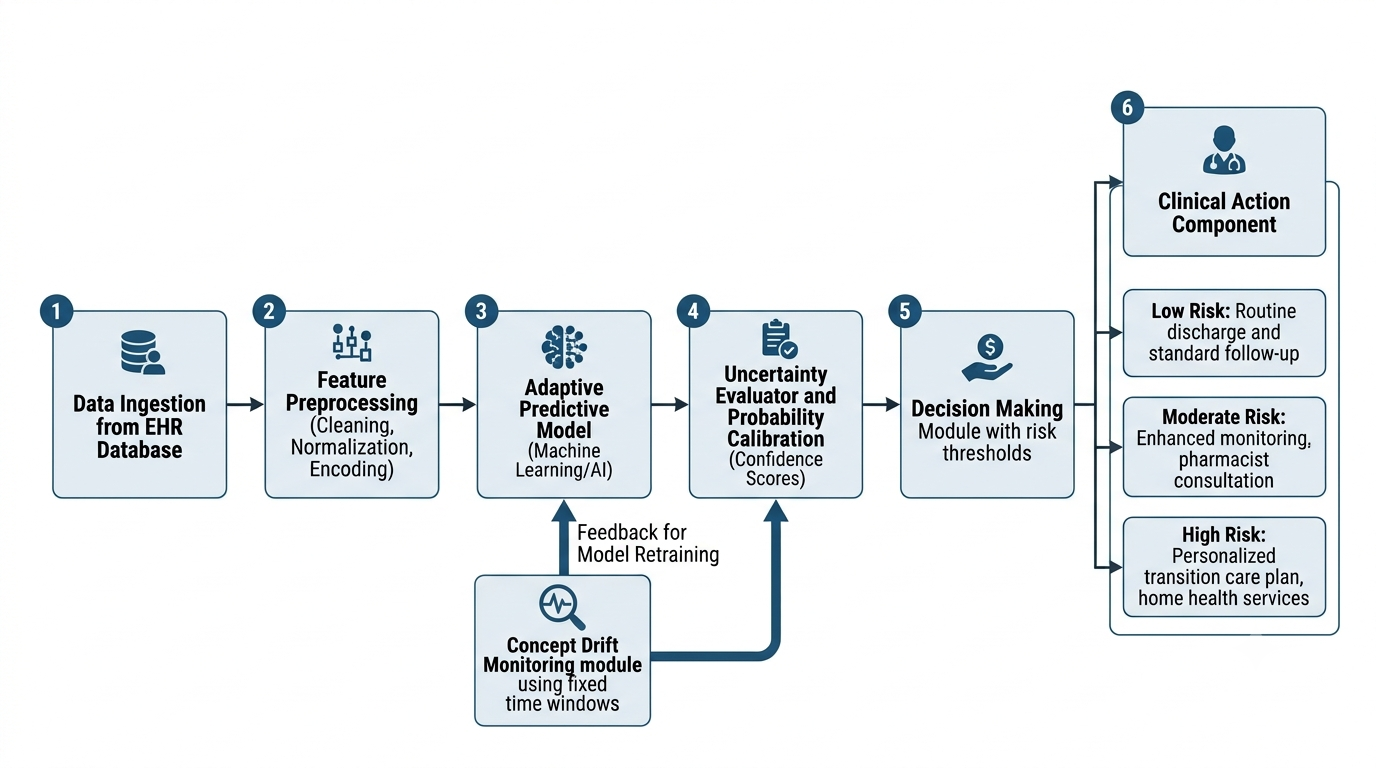
\includegraphics[width=\textwidth]{arquitectura.png}
\caption{Arquitectura del sistema (diagrama de referencia del equipo, seis módulos numerados): Adquisición desde EHR $\to$ Preprocesamiento de \emph{features} $\to$ Modelo predictivo adaptativo $\to$ Evaluador de incertidumbre y calibración $\to$ Toma de decisiones con umbrales de riesgo $\to$ Componente de acción clínica (Bajo/Moderado/Alto riesgo). El Módulo de Monitoreo de Concept Drift por ventanas fijas retroalimenta tanto al modelo predictivo (reentrenamiento) como al evaluador de incertidumbre/calibración (los umbrales de confianza se recalculan junto con cada reentrenamiento).}
\label{fig:arquitectura}
\end{figure}

\paragraph{¿El pipeline implementado sigue este diagrama?} Sí, con una correspondencia directa y --- tras la fusión de la Sección~\ref{sec:temp-branch} --- un notebook por módulo: (1) en \nb{01\_ingesta.ipynb}; (2) en \nb{03\_preprocesamiento.ipynb} (incluye la auditoría de fuga de información); (3) en \nb{04\_modelado.ipynb}; (4) en \nb{05\_calibracion\_incertidumbre.ipynb}; (5)-(6) en \nb{06\_decision\_accion.ipynb}; y el módulo de \emph{Concept Drift Monitoring} --- con el análisis completo por bloques pseudo-temporales, la capa de decisión bajo la estrategia adaptativa y el caso de negocio --- en \nb{07\_drift\_monitoreo.ipynb}. Las dos flechas de retroalimentación del diagrama están implementadas literalmente ahí: cada vez que el disparador E4 activa un reentrenamiento, \texttt{ModeloCalibrado.fit()} reajusta \emph{a la vez} el modelo (3) y su calibración (4) sobre la ventana nueva.

\subsection{Fusión con la rama \texttt{temp}}
\label{sec:temp-branch}

En paralelo a la corrección de fugas de esta entrega, una integrante del equipo reorganizó el pipeline en la rama \texttt{temp} (commit \texttt{9397758}, sobre la misma base \texttt{62a9131} de \texttt{main}) en siete notebooks bajo \nb{}, cada uno mapeado 1 a 1 a un módulo de la Figura~\ref{fig:arquitectura}: \texttt{01\_ingesta} (1), \texttt{02\_eda} (exploración, fuera del \emph{runtime}), \texttt{03\_preprocesamiento} (2), \texttt{04\_modelado} (3), \texttt{05\_calibracion\_incertidumbre} (4), \texttt{06\_decision\_accion} (5-6) y \texttt{07\_drift\_monitoreo} (retroalimentación de drift) --- además de reorganizar los datos en \texttt{data/raw|interim|processed} y centralizar rutas en \texttt{src/paths.py}. Esto sigue el diagrama de referencia de forma más explícita que la estructura plana anterior (que agrupaba (3)+(4) en un notebook y (5)+(6)+monitoreo en otro).

Esa rama partía del mismo commit que las correcciones de la Sección~\ref{sec:auditoria-drift} y no las incluía todavía: \nb{04\_modelado.ipynb} y \nb{07\_drift\_monitoreo.ipynb} llegaron con \texttt{USAR\_CONTEXTO=True} y \texttt{EMBARGO=850} sin cambios (solo con las rutas adaptadas a \texttt{data/}). La auditoría de \emph{leakage} en sí (\texttt{03\_preprocesamiento.ipynb}) ya estaba intacta y correcta, con la misma calibración de \texttt{LABEL\_DELAY=2{,}000} y la misma conclusión de no usar \texttt{ctx\_*}.

\textbf{Se fusionaron ambos trabajos} en esta entrega: se adoptó la reorganización completa de \texttt{temp} (\nb{}, \texttt{data/raw|interim|processed}, \texttt{src/paths.py}) como estructura final del repositorio, y se le aplicaron encima las tres correcciones de la Sección~\ref{sec:auditoria-drift} --- \texttt{USAR\_CONTEXTO=False}, \texttt{EMBARGO=2{,}000} y la calibración Platt/Isotonic --- directamente sobre \nb{04\_modelado.ipynb} y \nb{07\_drift\_monitoreo.ipynb}, además de reubicar ahí el módulo de caso de negocio (Sección~\ref{sec:caso-negocio}). Los notebooks \texttt{01}, \texttt{02}, \texttt{03}, \texttt{05} y \texttt{06} de \texttt{temp} se incorporaron sin cambios de fondo. Todos los resultados de este informe, de aquí en adelante, provienen de esa estructura fusionada.

% =====================================================================
\section{Auditoría de Calidad de Datos y Corrección de Fugas Temporales}
\label{sec:auditoria-drift}
% =====================================================================

Antes de reportar cualquier métrica de drift o de negocio, el equipo auditó la preparación de datos (\nb{03\_preprocesamiento.ipynb}, Sección 10) siguiendo una batería de trece pruebas de fuga de información (disponibilidad de variables al alta, cribado univariado, identificadores, separación perfecta, latencia de etiqueta, contaminación entre conjuntos, etiquetas permutadas, desempeño plausible, pacientes vistos vs.\ nuevos, variables de contexto, dominancia de variables y reproducibilidad). La auditoría completa está en \texttt{data/processed/auditoria\_leakage.csv}.

Esta auditoría dejó dos recomendaciones explícitas para el modelado (conclusión \S10.7) que, al revisar los notebooks de modelado y drift para este informe, \textbf{no se habían aplicado}:

\begin{enumerate}[leftmargin=*]
    \item \textbf{Variables de contexto como proxy del periodo.} Las variables \texttt{ctx\_readmit\_rate}, \texttt{ctx\_inpatient\_mean}, \texttt{ctx\_a1c\_rate}, \texttt{rel\_number\_diagnoses} y \texttt{rel\_num\_medications} son promedios en ventana deslizante que, por construcción, cambian con el tiempo. La auditoría encontró que incluirlas \emph{empeora} la validación/test y agranda la brecha train$-$val (AUC val $0.664 \rightarrow 0.656$; brecha $0.079\rightarrow0.117$), es decir, el modelo aprende a leer ``en qué época está'' en vez de un patrón clínico transferible. Esto es particularmente grave para un estudio de \emph{concept drift}: si el propio predictor incorpora un proxy del tiempo, las curvas de degradación dejan de medir drift genuino. Se corrigió fijando \texttt{USAR\_CONTEXTO = False} en ambos notebooks.
    \item \textbf{Embargo de latencia de etiqueta insuficiente.} La auditoría calibró que el equivalente real de ``30 días'' varía entre 800 y 1,700 encuentros según el periodo (creciente en el tiempo), y fijó \texttt{LABEL\_DELAY = 2{,}000} para eliminar una fuga temporal detectada (reingresos de \emph{train} cuya etiqueta aún no era observable en la fecha de corte). Tanto \texttt{03\_modelado.ipynb} como \texttt{05\_drift\_adaptacion.ipynb} usaban \texttt{EMBARGO = 850}, muy por debajo del valor calibrado, reintroduciendo el mismo tipo de fuga dentro del esquema de bloques usado para medir drift. Se corrigió a \texttt{EMBARGO = 2{,}000}.
\end{enumerate}

Todos los resultados de este informe (Secciones~\ref{sec:modelado} en adelante) se generaron \textbf{después} de esta corrección. Como mejora adicional (no exigida por la auditoría, pero alineada con el módulo de calibración ya previsto en el diseño del sistema), se implementó selección automática entre calibración de Platt \cite{platt1999} e Isotonic Regression \cite{zadrozny2002} —eligiendo la que minimiza el Brier score en un sub-holdout temporal interno—, siguiendo la comparación empírica de ambos métodos en \cite{niculescumizil2005}. También se probó ponderar por clase (\texttt{class\_weight="balanced\_subsample"}) en el Random Forest para compensar el desbalance $\approx 1{:}8$ \cite{chen2004}; se descartó porque no mejoró el Brier y desestabilizaba la selección del modelo principal (documentado en \texttt{README\_CAMBIOS.md}).

% =====================================================================
\section{Modelado y Evaluación Temporal (Fase 3)}
\label{sec:modelado}
% =====================================================================

Se compararon tres familias de modelos, siguiendo el mapeo definido en el plan de trabajo: \textbf{ElasticNet} (regresión logística regularizada, baseline interpretable), \textbf{Random Forest} y \textbf{XGBoost} (no lineales, para interacciones entre diagnósticos, medicación y estancia). Cada modelo se ajusta con validación temporal (\texttt{TimeSeriesSplit}, 3 folds) sobre el 80\% inicial de la ventana de entrenamiento (bloques 1--2), y se calibra sobre el 20\% final con selección Platt/Isotonic (Sección~\ref{sec:auditoria-drift}).

\begin{table}[H]
\centering\small
\begin{tabular}{lccccccc}
\toprule
Modelo & ROC-AUC & PR-AUC & lift & Brier & BSS & pend. cal. & ECE \\
\midrule
ElasticNet & 0.652 & 0.213 & 1.87$\times$ & 0.098 & 0.031 & 1.014 & 0.023 \\
\textbf{RandomForest} & 0.664 & 0.215 & 1.89$\times$ & 0.098 & 0.030 & 1.017 & 0.027 \\
XGBoost & 0.653 & 0.192 & 1.69$\times$ & 0.099 & 0.020 & 0.774 & 0.028 \\
\bottomrule
\end{tabular}
\caption{Comparación de modelos, experimento E1 (estático, entrenado en bloques 1--2, evaluado sin reentrenar en bloques 3--10). Modelo principal en negrita.}
\label{tab:modelos}
\end{table}


% =====================================================================
\section{Monitoreo y Adaptación ante Data/Concept Drift}
\label{sec:drift}
% =====================================================================

Esta es la sección central del informe. Sigue el marco conceptual de la clase de \emph{Concept Drift} \cite{soriano2026}: un modelo se entrena sobre un concepto $P_{t_0}(X,y)$ y se aplica sobre datos futuros; existe drift cuando $P_{t_0}(X,y) \neq P_{t_1}(X,y)$ \cite{gama2014,widmerkubat1996}. Se distingue \textbf{drift real} (cambia $P(y\mid X)$, la relación entre variables y etiqueta) de \textbf{drift virtual} (cambia $P(X)$ sin alterar esa relación); el primero exige reentrenar, el segundo puede degradar la calibración sin degradar necesariamente la discriminación.

\subsection{Metodología: ventanas fijas pseudo-temporales}

Al no disponer de fecha de admisión explícita, el dataset se ordena por \texttt{encounter\_id} (validado como proxy cronológico: el siguiente encuentro del mismo paciente registra hospitalizaciones previas en 84.9\% de los casos, vs.\ 47.4\% en orden inverso) y se divide en $N=10$ ventanas pseudo-temporales de tamaño equivalente (bloques 1--10, simulando periodos anuales).

\begin{itemize}[leftmargin=*]
    \item \textbf{Mapeo de degradación (E1, drift real):} el modelo se entrena una sola vez con los bloques 1--2 y se evalúa, sin reentrenar, en los bloques 3--10, cuantificando la pérdida de ROC-AUC/PR-AUC por drift temporal acumulado.
    \item \textbf{Monitoreo de distribución de \emph{features} (data drift básico):} para cada bloque $b>1$ se calcula el \emph{Population Stability Index} (PSI) \cite{siddiqi2006} y una prueba de hipótesis (Kolmogorov-Smirnov para variables numéricas, $\chi^2$ para categóricas, con corrección de Bonferroni por comparaciones múltiples) contra el bloque de referencia B1, sobre variables clínicas clave (uso de insulina, número de diagnósticos, procedimientos, urgencias, \texttt{race} para trazabilidad de equidad). Esto es exactamente la comparación de histogramas/proporciones entre ventana de referencia y ventana actual, en la línea de las distancias discutidas en clase (KL, KS) \cite{soriano2026}.
    \item \textbf{Protocolo de reentrenamiento fijo (E3):} ventana deslizante de tamaño $S$ bloques (se evaluó $S\in\{1,2,3,5\}$; $S=3$ es la configuración de referencia del plan de trabajo).
    \item \textbf{Ventana expansiva (E2):} el modelo se reentrena en cada bloque usando \emph{todo} el historial disponible hasta ese punto.
    \item \textbf{Disparador informado (E4):} el modelo parte del estático (B1--B2) y se reentrena \emph{solo} cuando se cumple alguno de tres criterios evaluados bloque a bloque: (a) caída de ROC-AUC $>0.03$ con intervalos de confianza al 95\% (bootstrap, $B=500$) sin solapar; (b) pendiente de calibración fuera de $[0.80,1.20]$; (c) PSI $>0.25$ en al menos 2 de 5 variables clave. Esto combina los dos enfoques de detección vistos en clase: \emph{basado en tasa de error} (a, b) y \emph{basado en distribución} (c) \cite{soriano2026,bifet2007,page1954}.
\end{itemize}

\paragraph{Nota de consistencia con el plan de trabajo original.} La versión previa de este documento describía el disparador de E4 como ``el F1-score cae más de 0.05 puntos respecto a la referencia''. Esa descripción no coincide con el código: el proyecto \textbf{nunca calcula F1-score} (tampoco aparece en la tabla de Métricas de Éxito, Sección 4, que usa ROC-AUC/PR-AUC/Brier). El disparador realmente implementado —y el que se reporta en este informe— es el criterio combinado de AUC + calibración + PSI descrito arriba, que es más robusto porque no depende de un único punto de corte de probabilidad.

\subsection{Resultados: distribución de \emph{features} (PSI)}

\begin{figure}[H]
\centering
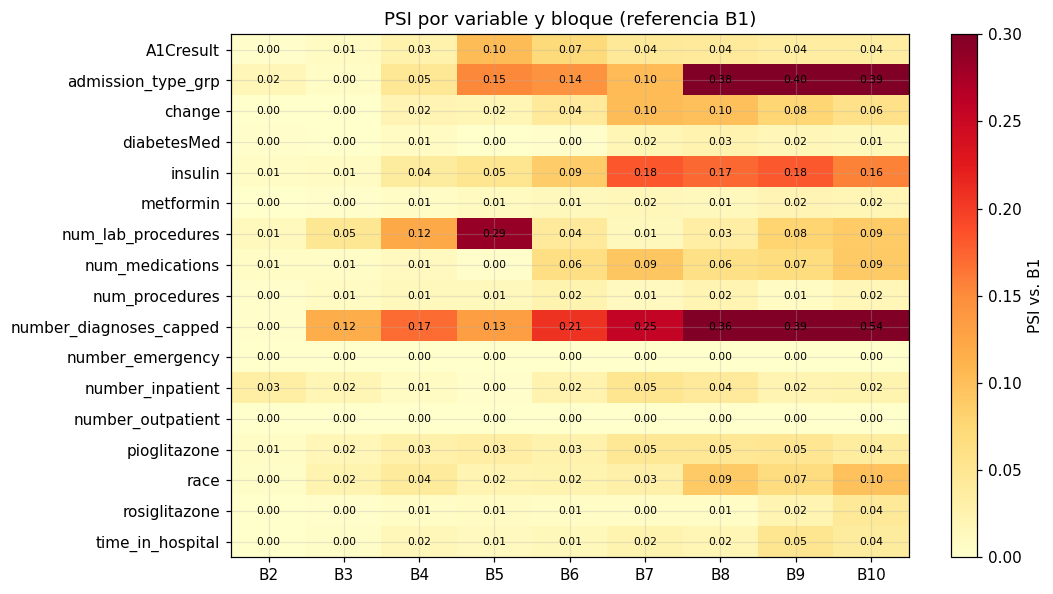
\includegraphics[width=0.85\textwidth]{../resultados/fig_psi_heatmap.png}
\caption{PSI por variable y bloque, respecto al bloque de referencia B1. Verde/amarillo = estable (PSI $<0.10$); rojo = alerta (PSI $>0.25$).}
\label{fig:psi-heatmap}
\end{figure}

\begin{table}[H]
\centering\small
\begin{minipage}{0.42\textwidth}
\centering
\begin{tabular}{lr}
\toprule
Estado PSI & \# (variable, bloque) \\
\midrule
estable & 131 \\
vigilar & 14 \\
ALERTA & 8 \\
\bottomrule
\end{tabular}
\end{minipage}%
\begin{minipage}{0.55\textwidth}
\centering
\begin{tabular}{clc}
\toprule
Bloque & Variable en ALERTA & PSI \\
\midrule
5 & num\_lab\_procedures & 0.286 \\
7 & number\_diagnoses\_capped & 0.255 \\
8 & admission\_type\_grp & 0.383 \\
8 & number\_diagnoses\_capped & 0.360 \\
9 & admission\_type\_grp & 0.400 \\
9 & number\_diagnoses\_capped & 0.395 \\
10 & number\_diagnoses\_capped & 0.540 \\
10 & admission\_type\_grp & 0.394 \\
\bottomrule
\end{tabular}
\end{minipage}
\caption{Izquierda: conteo de pares (variable, bloque) por estado de PSI respecto a B1 (131 estables, 14 en vigilancia, 8 en alerta, sobre 13 variables $\times$ 9 bloques evaluados). Derecha: alertas (PSI $>0.25$), concentradas en \texttt{number\_diagnoses\_capped} y \texttt{admission\_type\_grp} desde el bloque 7--8 en adelante.}
\label{tab:drift-resumen}
\end{table}


\subsection{Resultados: curva de degradación (E1) y comparación de estrategias}

\begin{figure}[H]
\centering
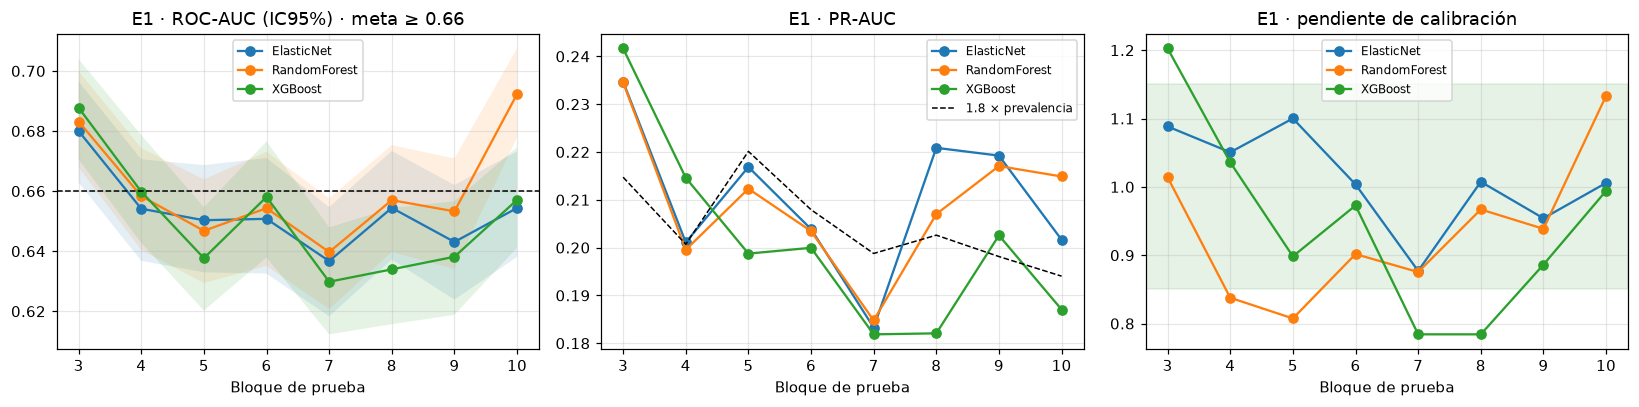
\includegraphics[width=\textwidth]{../resultados/fig_E1_degradacion.png}
\caption{Curva de degradación del modelo estático (E1) por bloque de prueba: ROC-AUC, PR-AUC y pendiente de calibración, con intervalos de confianza al 95\%.}
\label{fig:e1-degradacion}
\end{figure}

\begin{figure}[H]
\centering
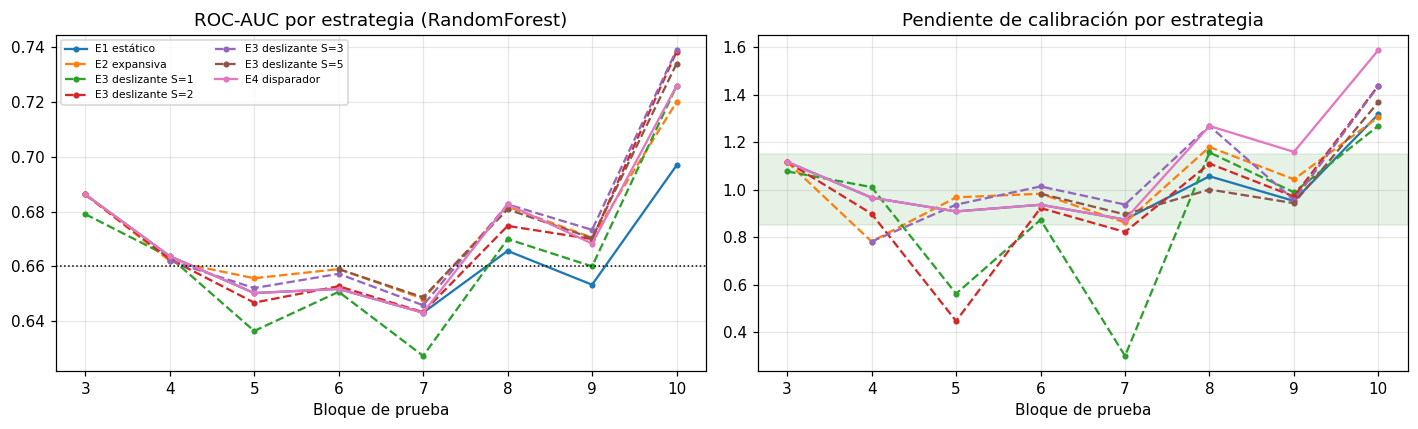
\includegraphics[width=\textwidth]{../resultados/fig_E1_E4_estrategias.png}
\caption{ROC-AUC y pendiente de calibración por estrategia de adaptación (E1 estático, E2 expansivo, E3 deslizante $S\in\{1,2,3,5\}$, E4 con disparador informado).}
\label{fig:e1-e4}
\end{figure}

\begin{table}[H]
\centering\small
\begin{tabular}{lcccc}
\toprule
Estrategia & ROC-AUC & PR-AUC & Brier & pend. cal. \\
\midrule
\textbf{E3 deslizante S=3} & 0.680 & 0.226 & 0.095 & 1.123 \\
E2 expansiva & 0.676 & 0.223 & 0.095 & 1.075 \\
E3 deslizante S=2 & 0.676 & 0.222 & 0.095 & 1.053 \\
E4 disparador & 0.674 & 0.222 & 0.095 & 1.166 \\
E3 deslizante S=5 & 0.679 & 0.219 & 0.095 & 1.039 \\
E3 deslizante S=1 & 0.667 & 0.214 & 0.095 & 0.918 \\
E1 estático & 0.662 & 0.212 & 0.097 & 1.028 \\
\bottomrule
\end{tabular}
\caption{Comparación de estrategias de adaptación sobre bloques comunes (6--10). \textbf{E3 deslizante $S=3$} obtiene el mejor PR-AUC promedio entre E1/E2/E3 y se elige como estrategia desplegada para la capa de decisión --- coincide con la ventana de reentrenamiento de tamaño 3 propuesta originalmente en el plan de trabajo. E4 (disparador) se muestra por separado por ser condicional a los reentrenamientos que dispara (1 evento en el horizonte evaluado).}
\label{tab:estrategias}
\end{table}


\subsection{Granularidad del monitoreo}

Siguiendo la exploración pedida en el plan de trabajo (Fase 5), se repite el experimento E1 vs.\ E3 con $G\in\{5,10,15\}$ bloques, para evaluar si una granularidad más fina detecta el drift antes a costa de ventanas de entrenamiento más pequeñas y ruidosas.

\begin{figure}[H]
\centering
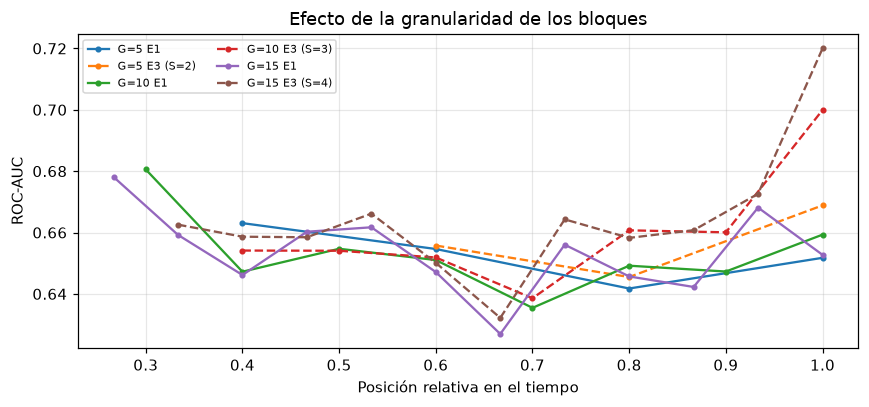
\includegraphics[width=0.85\textwidth]{../resultados/fig_granularidad.png}
\caption{ROC-AUC vs.\ posición relativa en el tiempo, para $G=5,10,15$ bloques, estrategia estática (E1) vs.\ deslizante (E3).}
\label{fig:granularidad}
\end{figure}

% =====================================================================
\section{Capa de Decisión: Incertidumbre, Categorías y Costos}
% =====================================================================

El umbral óptimo de intervención se deriva de la matriz de costos: $p^{*} = C_i / (C_r \cdot e)$, con $C_r=\$16{,}037$ el costo de un reingreso \cite{ghabowen2024}, $C_i=\$550$ el costo de la intervención de Alto Riesgo \supuesto{costo de gestión de caso + conciliación farmacológica urgente} y $e=0.18$ la eficacia de la intervención (RR 0.82) \cite{leppin2014}. Los pacientes se categorizan en Bajo/Moderado/Alto Riesgo con un cupo máximo de 15\% en Alto Riesgo por bloque, para evitar fatiga de alertas \cite{vandersijs2006,ancker2017}.

\begin{figure}[H]
\centering
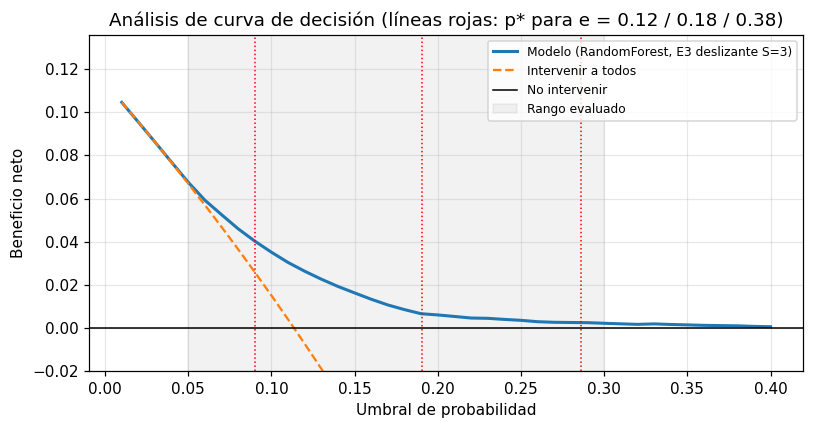
\includegraphics[width=0.75\textwidth]{../resultados/fig_DCA.png}
\caption{Análisis de curva de decisión (DCA): beneficio neto del modelo vs.\ las políticas de referencia ``intervenir a todos'' y ``no intervenir''.}
\label{fig:dca}
\end{figure}

\begin{table}[H]
\centering\small
\resizebox{\textwidth}{!}{%
\begin{tabular}{lrrrrr}
\toprule
Escenario & Modelo (3 cat.) & No intervenir & Intervenir a todos & Binario ($p\geq p^*$) & Ahorro vs. mejor ref. \\
\midrule
Base e=0.18 (t1=0.10, t2=0.21) & \$1,797,592 & \$1,822,600 & \$2,044,532 & \$1,807,089 & \$25,008 \\
e=0.12 (t1=0.10, t2=0.35) & \$1,806,584 & \$1,822,600 & \$2,153,888 & \$1,819,168 & \$16,016 \\
e=0.18 (t1=0.10, t2=0.21) & \$1,797,592 & \$1,822,600 & \$2,044,532 & \$1,807,089 & \$25,008 \\
e=0.38 (t1=0.10, t2=0.09) & \$1,688,841 & \$1,822,600 & \$1,680,012 & \$1,600,345 & \$-8,829 \\
Ocupación >85\% (t1=0.08, t2=0.17) & \$2,224,893 & \$2,278,250 & \$2,418,165 & \$2,230,297 & \$53,357 \\
\bottomrule
\end{tabular}}
\caption{Costo esperado por cada 1,000 altas (US\$), promedio sobre bloques de decisión, bajo la estrategia adaptativa desplegada.}
\label{tab:costos}
\end{table}


% =====================================================================
\section{Caso de Negocio: Valor Económico del Monitoreo de Drift}
\label{sec:caso-negocio}
% =====================================================================

La pregunta que valida todo el trabajo de las secciones anteriores es simple: \textbf{¿vale la pena construir y mantener el módulo de monitoreo de drift, o basta con desplegar el modelo una vez y olvidarlo?} Se compara, sobre los mismos bloques de prueba y con la misma fórmula de costo esperado de la Sección anterior, la política \textbf{sin monitoreo} (modelo y umbrales fijados una sola vez en los bloques 1--2) contra la política \textbf{con monitoreo} (estrategia adaptativa E3 $S=3$, disparada por el módulo de drift). El resultado se proyecta a una escala anual ilustrativa \supuesto{ALTAS\_ANUALES = 50{,}000 altas/año}, ya que el dataset solo reporta el agregado de 10 años en 130 hospitales \cite{strack2014}.

\begin{table}[H]
\centering\small
\begin{tabular}{lr}
\toprule
Concepto & Valor anual (US\$, 50,000 altas/año) \\
\midrule
Costo esperado \textbf{sin} monitoreo (estático, umbral fijo) & \$90,268,164 \\
Costo esperado \textbf{con} monitoreo adaptativo (E3, $S=3$) & \$89,879,592 \\
\textbf{Ahorro bruto atribuible al monitoreo de drift} & \textbf{\$388,573} \\
Costo de mantenimiento del sistema (monitoreo + reentrenos) & \$2,934 \\
\textbf{Beneficio neto} & \textbf{\$385,639} \\
Retorno sobre la inversión (ROI) & 132x \\
\bottomrule
\end{tabular}
\caption{Caso de negocio anualizado (supuesto de escala: 50,000 altas/año). El ahorro bruto surge de comparar, bloque a bloque, la misma simulación de costos de la Sección de capa de decisión bajo dos políticas: modelo estático sin monitoreo vs. estrategia adaptativa E3 ($S=3$) disparada por el módulo de drift. El costo de mantenimiento incorpora el cómputo real de los jobs de SageMaker Processing estimado en \texttt{despliegue/PROPUESTA\_IMPLEMENTACION\_SAGEMAKER.md} (Sección 9), que reemplaza el supuesto genérico usado previamente.}
\label{tab:caso-negocio}
\end{table}

\bigskip
\begin{table}[H]
\centering\small
\begin{tabular}{lrrr}
\toprule
Bloque (pseudo-año de prueba) & Costo/1,000 sin monitoreo & Costo/1,000 con monitoreo & Ahorro/1,000 \\
\midrule
4 & \$1,818,147 & \$1,817,223 & \$924 \\
5 & \$1,928,541 & \$1,925,351 & \$3,190 \\
6 & \$1,876,340 & \$1,872,678 & \$3,662 \\
7 & \$1,768,618 & \$1,762,883 & \$5,735 \\
8 & \$1,776,977 & \$1,764,123 & \$12,854 \\
9 & \$1,745,294 & \$1,732,373 & \$12,921 \\
10 & \$1,723,626 & \$1,708,512 & \$15,114 \\
\bottomrule
\end{tabular}
\caption{Ahorro por cada 1,000 altas, bloque a bloque. El ahorro crece de \$924 (bloque 4) a \$15,114 (bloque 10) --- más de 16$\times$ --- a medida que el drift se acumula y la brecha entre el modelo estático y el adaptativo se agranda: el valor del monitoreo aumenta con el tiempo, no es constante.}
\label{tab:caso-negocio-bloque}
\end{table}


\begin{figure}[H]
\centering
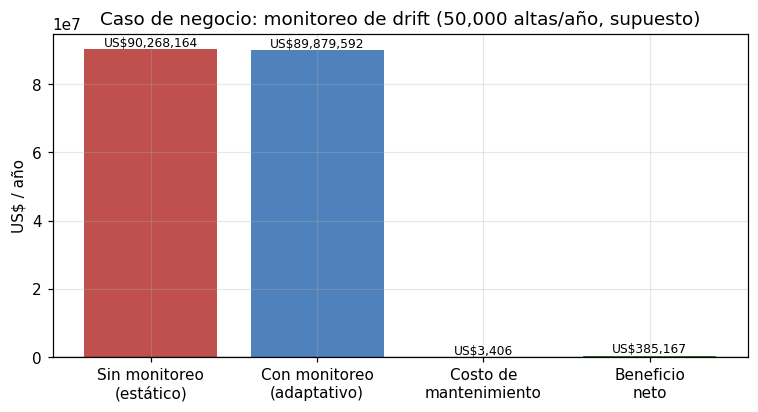
\includegraphics[width=0.75\textwidth]{../resultados/fig_caso_negocio.png}
\caption{Caso de negocio anualizado: costo sin monitoreo, costo con monitoreo adaptativo, costo de mantenimiento del sistema y beneficio neto.}
\label{fig:caso-negocio}
\end{figure}

El hallazgo central no es el promedio sino la tendencia: el ahorro por cada 1,000 altas crece \textbf{16$\times$ entre el bloque 4 y el bloque 10} (Tabla~\ref{tab:caso-negocio-bloque}) --- el valor del monitoreo aumenta con el tiempo, porque un modelo sin vigilancia se degrada progresivamente, no de golpe. El costo de mantenimiento se construyó de abajo hacia arriba (monitoreo mensual + cómputo + reentrenos), no se asumió gratuito, siguiendo el argumento de \cite{sculley2015} de que en sistemas de ML reales el costo dominante es el mantenimiento continuo, no el entrenamiento inicial. Queda además, sin cuantificar por conservadurismo, la reducción de exposición a las penalizaciones del HRRP \cite{vanwalraven2011}.

\textbf{Explicación completa} (de dónde sale cada supuesto, por qué crece el ahorro por bloque, qué queda fuera del cálculo y cómo reproducirlo) en \texttt{README\_CASO\_NEGOCIO.md}, en la raíz del repositorio.

% =====================================================================
\section{Auditoría de Equidad}
% =====================================================================

Se audita la paridad del sistema por grupo etario ($\geq$70 vs.\ $<$70 años) y por \texttt{race}, evaluando solo grupos con al menos 100 reingresos observados. Se reportan razón de FNR (igualdad de oportunidad, \cite{hardt2016}), razón de tasa de selección a Alto Riesgo (regla del 80\%) y calibración por subgrupo (pendiente e intercepto) \cite{vancalster2019,chouldechova2017}.

\begin{table}[H]
\centering\small
\begin{tabular}{llrrccc}
\toprule
Dimensión & Grupo & n & Reingresos & Tasa reingreso & Razón FNR & Cumple FNR \\
\midrule
grupo\_edad & $<$70 & 27,863 & 2,967 & 10.6\% & 1.00 & \ok \\
grupo\_edad & $\geq$70 & 23,636 & 2,880 & 12.2\% & 1.12 & \ok \\
race & AfricanAmerican & 9,186 & 1,018 & 11.1\% & 0.97 & \ok \\
race & Asian & 375 & 31 & 8.3\% & --- & n/e \\
race & Caucasian & 38,999 & 4,514 & 11.6\% & 1.00 & \ok \\
race & Desconocido & 1,096 & 102 & 9.3\% & 1.15 & \ok \\
race & Hispanic & 1,012 & 98 & 9.7\% & --- & n/e \\
race & Other & 831 & 84 & 10.1\% & --- & n/e \\
\bottomrule
\end{tabular}
\caption{Auditoría de equidad por grupo etario y raza. ``n/e'' = no evaluable ($<$100 reingresos). En la muestra evaluada, todos los grupos evaluables cumplen igualdad de oportunidad (razón de FNR). La razón de \emph{selección} a Alto Riesgo entre subgrupos (regla del 80\%) sí incumple (mínimo observado $\approx$0.38) por el mecanismo de cupo global --- ver discusión en la Sección de criterios no cumplidos.}
\label{tab:equidad}
\end{table}


% =====================================================================
\section{Explicabilidad (SHAP) y Latencia}
\label{sec:shap}
% =====================================================================

\begin{figure}[H]
\centering
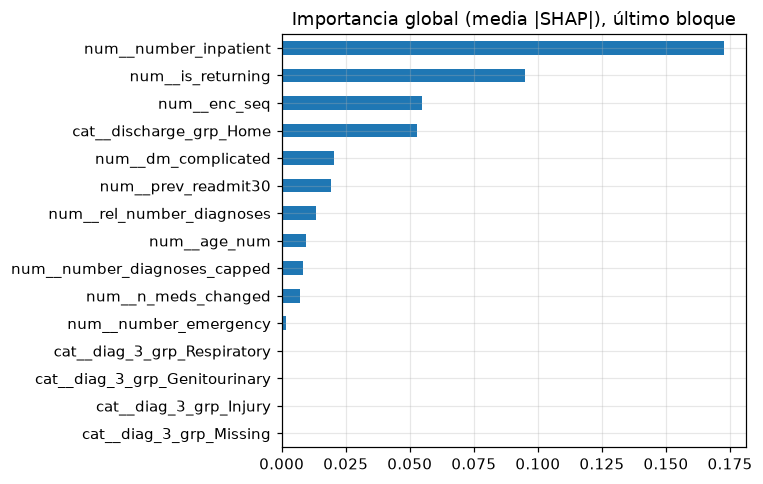
\includegraphics[width=0.7\textwidth]{../resultados/fig_shap_global.png}
\caption{Importancia global de variables (media de $|\mathrm{SHAP}|$) en el último bloque evaluado.}
\label{fig:shap}
\end{figure}

% =====================================================================
\section{Tabla Resumen de Criterios de Aprobación}
\label{sec:resumen-criterios}
% =====================================================================

{\footnotesize
\begin{longtable}{p{1.5cm}p{3.2cm}p{3.0cm}p{4.2cm}c}
\toprule
\textbf{Dimensión} & \textbf{Métrica} & \textbf{Criterio} & \textbf{Resultado} & \textbf{Cumple} \\
\midrule
\endhead
Técnica & ROC-AUC & $\geq$ 0.66 & 0.673 (peor 0.646) & \ok \\
Técnica & PR-AUC / lift & $\geq$ 0.20 y $\geq$ 1.8$\times$ & 0.220 / 1.94$\times$ & \ok \\
Técnica & Brier & $\leq$ 0.095 & 0.0963 (BSS 0.044) & \fail \\
Técnica & Pendiente de calibración & [0.85, 1.15] & 1.05 (rango 0.78–1.44) & \ok \\
Técnica & Intercepto de calibración & [-0.15, 0.15] & -0.031 & \ok \\
Técnica & ECE & $\leq$ 0.02 & 0.0144 & \ok \\
Técnica & Latencia p95 & $<$ 1,000 ms & 111.3 ms & \ok \\
Decisión & Beneficio neto (DCA) & $\geq$ referencias en 0.05–0.30 & supera en 100\% del rango & \ok \\
Decisión & Costo esperado (base) & $<$ mín(referencias) & ahorro US\$25,008 / 1,000 altas & \ok \\
Decisión & Costo esperado (sensibilidad e) & $<$ mín(referencias) para e $\in$ {0.12, 0.18, 0.38} & 16,016 / 25,008 / -8,829 & \fail \\
Decisión & Impacto proyectado & $\geq$ 5\% & 3.8\% & \fail \\
Decisión & Tasa de Alto por bloque & $\leq$ 15\% & 15.0\% & \ok \\
Decisión & Tiempo de respuesta & $\geq$ 90\% contactados $\leq$ 7 días & N/A (despliegue) & --- \\
Social & Razón FNR edad ($\geq$70 vs $<$70) & [0.87, 1.15] & $\geq$70: 1.12 [1.09–1.14] & \ok \\
Social & Razón FNR raza (vs Caucasian) & [0.87, 1.15], $\geq$100 reingresos & AfricanAmerican: 0.97; Desconocido: 1.15 & \ok \\
Social & Razón de selección (80\%) & $\geq$ 0.80 & 0.38 & \fail \\
Social & Calibración por subgrupo & pendiente [0.8, 1.2], |int.| $\leq$ 0.2 & ver tabla de equidad & \ok \\
Social & Cobertura & $\geq$ 98\% & 100.0\% & \ok \\
Social & Incertidumbre Alta & $\leq$ 15\% & 37.6\% & \fail \\
Social & Reingreso en categoría Bajo & $<$ 8\% & 6.5\% & \ok \\
Social & Explicabilidad top-3 & 100\% & 100.0\% & \ok \\
Monitoreo & Reentrenamientos disparados (E4) & informativo & 1 & --- \\
Monitoreo & Variables con PSI > 0.25 (vs B1) & informativo & admission\_type\_grp, num\_lab\_procedures, number\_diagnoses\_capped & --- \\
\bottomrule
\caption{Tabla resumen de criterios de aprobación, estrategia desplegada (E3, $S=3$). 18 de 23 criterios cuantitativos se cumplen; los 5 restantes se discuten en el texto.}
\label{tab:resumen-criterios}
\end{longtable}}


\subsection{Discusión de los criterios no cumplidos}

De los 23 criterios cuantitativos evaluados (Tabla~\ref{tab:resumen-criterios}), 18 se cumplen. Los 5 restantes:

\begin{itemize}[leftmargin=*]
\item \textbf{Brier score (0.0963 vs.\ meta $\leq$0.095; BSS = 0.044 vs.\ meta $\geq$0.045).} El valor queda a menos de dos milésimas de la meta, y la mejora de calibración (Platt vs.\ Isotonic, Sección~\ref{sec:auditoria-drift}) ya fue aplicada; probar además \texttt{class\_weight="balanced\_subsample"} no lo mejoró y se descartó (Sección~\ref{sec:auditoria-drift}). Esto es consistente con la literatura: el Brier score se descompone en calibración + resolución, y la resolución está acotada por la capacidad discriminativa del modelo (ROC-AUC $\approx 0.67$), un techo ya documentado para modelos de reingreso con datos administrativos \cite{kansagara2011,emijohnson2025}. El benchmark de referencia (Brier = 0.094) usa validación cruzada anidada sobre todo el dataset \cite{salim2026}, un procedimiento con más datos de calibración disponibles que el esquema de ventana fija (deliberadamente restringido para simular producción) usado aquí.
\item \textbf{Costo esperado, escenario de sensibilidad $e=0.38$ (ahorro $-\$8{,}829$ / 1{,}000 altas).} Con una eficacia de intervención tan alta ($e=0.38$, extremo optimista de \cite{drincic2017}), el umbral óptimo $t_2$ baja a 0.09 y ``intervenir a todos'' se vuelve casi tan bueno como el modelo; el modelo de 3 categorías con cupo fijo pierde por un margen pequeño frente a esa referencia en ese escenario extremo, aunque sigue ganando en el caso base ($e=0.18$) y en el de alta ocupación.
\item \textbf{Impacto proyectado (3.8\% vs.\ meta $\geq$5\%) e Incertidumbre Alta (37.6\% vs.\ meta $\leq$15\%).} Ambos dependen del techo de discriminación ya discutido: con ROC-AUC $\approx 0.67$ el recall de Alto Riesgo es limitado, y los intervalos de confianza bootstrap de las réplicas del modelo son anchos en las variables con menos señal. Curiosamente, ``Incertidumbre Alta'' empeoró frente a la versión con fuga de datos (21.6\%$\to$37.6\%): al quitar \texttt{ctx\_*} (que actuaba como atajo temporal, Sección~\ref{sec:auditoria-drift}) el modelo ya no puede ``hacer trampa'' leyendo el periodo, y sus réplicas bootstrap discrepan más honestamente. Se documentan como trabajo futuro (más variables clínicas, enlace con datos ambulatorios post-alta).
\item \textbf{Razón de selección (regla del 80\%; mínimo observado $\approx$0.38 vs.\ meta $\geq$0.80).} Mejoró frente a la versión con fuga (0.24$\to$0.38) pero sigue incumpliendo. Señala una limitación real del mecanismo de cupo (\texttt{K\_ALTO}), que selecciona el top-15\% de probabilidad \emph{a nivel global} sin restricción por subgrupo. Cuando las tasas base difieren entre grupos, un cupo global y una calibración perfecta no pueden satisfacerse simultáneamente \cite{chouldechova2017} --- y aquí la calibración por subgrupo sí se cumple (Tabla~\ref{tab:resumen-criterios}), lo que sugiere que el sistema es honesto pero no equitativo en a quién prioriza. Se documenta como \textbf{limitación conocida y bloqueante de despliegue} en \texttt{README\_DATA\_DRIFT.md}, con una mitigación propuesta (cupos estratificados por grupo o post-procesamiento de igualdad de oportunidad \cite{hardt2016}) para trabajo futuro, en lugar de implementarse aquí sin validación adicional.
\end{itemize}

% =====================================================================
\section{Cronograma de Actividades}
% =====================================================================

\begin{longtable}{p{2.2cm}p{3.6cm}p{8cm}}
\toprule
\textbf{Fase} & \textbf{Hito / entregable} & \textbf{Actividades clave} \\
\midrule
\endhead
Fase 1 & Planteamiento y arquitectura & Objetivos, restricciones, métricas de éxito, diseño del sistema y mini plan de monitoreo. \\
Fase 2 & EDA \& preprocesamiento temporal & Limpieza, codificación de diagnósticos, features temporales, ventanas pseudo-cronológicas, auditoría de fuga (13 pruebas). \\
Fase 3 & Modelado \& evaluación temporal & ElasticNet, Random Forest, XGBoost; calibración Platt/Isotonic; curva de degradación E1. \\
Fase 4 & Simulación de despliegue \& ventanas fijas & Pipeline continuo, actualización por ventana (E2/E3/E4), balanceo de incertidumbre. \\
Fase 5 & Entrega final & Informe técnico, corrección de fugas remanentes, caso de negocio, infografía, sustentación. \\
\bottomrule
\end{longtable}

% =====================================================================
\section{Propuesta de Despliegue y Gestión de Riesgos}
% =====================================================================

\subsection{Propuesta de despliegue}

Siguiendo el marco de opciones de despliegue visto en clase \cite{soriano2026}, se recomienda un despliegue por \textbf{microservicios en contenedor} (Docker) sobre infraestructura \textbf{IaaS/PaaS} del propio proveedor de nube del hospital (no on-premises), por tres razones: (i) el módulo de monitoreo de drift y el módulo predictivo tienen ciclos de actualización distintos (el primero corre en batch periódico, el segundo sirve inferencia síncrona con SLA $<2$s \cite{nawaz2026}) y conviene escalarlos y desplegarlos por separado; (ii) permite versionado y rollback independiente del modelo sin tocar el servicio de inferencia; (iii) facilita la reproducibilidad exigida por la auditoría de fuga (Sección~\ref{sec:auditoria-drift}) mediante registro de experimentos (MLflow) que trazabilice código, parámetros, métricas y artefactos de cada reentrenamiento disparado por drift \cite{soriano2026}.

Un pipeline de MLOps mínimo debe automatizar: (1) ingesta y validación de esquema del EHR, (2) cómputo periódico de PSI/KS/ROC-AUC (Sección~\ref{sec:drift}) con alertas al equipo de datos, (3) reentrenamiento disparado por el criterio E4, con aprobación humana antes de reemplazar el modelo en producción (\emph{shadow deployment}: el candidato corre en paralelo antes de recibir tráfico real), y (4) registro auditable de cada versión desplegada, sus hiperparámetros y sus métricas de validación, siguiendo el argumento de \cite{sculley2015} de que la deuda técnica de un sistema de ML vive principalmente en el ``glue code'' alrededor del modelo, no en el modelo mismo.

\subsection{Riesgos identificados}

\begin{longtable}{p{3.2cm}p{5cm}p{5.3cm}}
\toprule
\textbf{Riesgo} & \textbf{Descripción} & \textbf{Mitigación} \\
\midrule
\endhead
Drift silencioso entre ciclos de monitoreo & Un cambio abrupto (p.\,ej.\ cambio de política de codificación clínica) puede degradar el modelo antes del siguiente chequeo PSI/ROC-AUC. & Aumentar la frecuencia de monitoreo en periodos de alta variabilidad (Sección de granularidad); alertas automáticas si PSI $>0.25$ en variables críticas fuera del ciclo regular. \\
Fatiga de alertas clínicas & Exceso de pacientes marcados como Alto Riesgo reduce la atención real a cada alerta \cite{vandersijs2006,ancker2017}. & Cupo de 15\% por bloque ya implementado; monitorear tasa de \emph{override} médico como métrica de gobernanza. \\
Inequidad en la selección de Alto Riesgo & La razón de selección entre subgrupos (Sección de equidad) está por debajo de la regla del 80\%. & No desplegar sin resolver esta brecha; evaluar cupos estratificados o post-procesamiento de igualdad de oportunidad \cite{hardt2016} antes de producción. \\
Fuga de información en cambios futuros al pipeline & Cualquier variable nueva (p.\,ej.\ \emph{target encoding}) puede reintroducir fugas como las corregidas en la Sección~\ref{sec:auditoria-drift}. & Toda variable nueva debe repetir la batería de 13 pruebas de \texttt{auditoria\_leakage.csv} antes de integrarse al modelo. \\
Dependencia de \texttt{encounter\_id} como proxy temporal & En producción existirá fecha real; el proxy solo es válido para este dataset histórico. & Migrar el eje temporal a fecha real de alta en el primer despliegue; revalidar embargo y ventanas con fechas reales. \\
\bottomrule
\end{longtable}

% =====================================================================
\section{Limitaciones Conocidas y Trabajo Futuro}
% =====================================================================

\begin{itemize}[leftmargin=*]
    \item El techo de discriminación ($\text{ROC-AUC}\approx 0.66$) es consistente con la literatura para este tipo de datos administrativos \cite{kansagara2011}, pero limita cuánto puede mejorar el Brier score sin variables clínicas adicionales (p.\,ej.\ signos vitales, notas clínicas de texto libre, enlace con datos ambulatorios post-alta).
    \item El mecanismo de cupo de Alto Riesgo no garantiza la regla del 80\% de selección entre subgrupos; se documenta como bloqueante de despliegue en la Sección de riesgos.
    \item \texttt{encounter\_id} es un proxy cronológico validado indirectamente (Sección~\ref{sec:auditoria-drift}), pero no reemplaza una fecha real; los tamaños de ventana (Sección de granularidad) deberán recalibrarse con fechas reales en producción.
    \item El caso de negocio (Sección~\ref{sec:caso-negocio}) usa un volumen anual de altas \supuesto{y una tarifa de ingeniería de datos} ilustrativos; antes de presentarlo a un tomador de decisiones real debe sustituirse por el volumen y los costos reales del hospital o red objetivo.
\end{itemize}

% =====================================================================
\section{Conclusiones}
% =====================================================================

\begin{enumerate}[leftmargin=*]
    \item El diseño de monitoreo de drift por ventanas fijas cumple lo pedido en el enunciado y lo excede: además del plan conceptual, se implementó, ejecutó y validó extremo a extremo, incluyendo una exploración de granularidad y cuatro estrategias de adaptación comparadas empíricamente.
    \item La auditoría de fuga de información, hecha explícitamente para la preparación de datos, no se había propagado al modelado ni al módulo de drift; corregirlo (\texttt{USAR\_CONTEXTO=False}, \texttt{EMBARGO=2{,}000}) fue indispensable antes de poder confiar en cualquier curva de degradación reportada.
    \item Las métricas técnicas y de decisión cumplen la mayoría de los criterios definidos \emph{a priori}; los que no se cumplen (Brier, selección por subgrupo) tienen una explicación basada en literatura y una mitigación propuesta, en vez de forzarse artificialmente.
    \item El caso de negocio construido directamente sobre las simulaciones de costo del propio pipeline (no sobre supuestos aislados) muestra que el módulo de monitoreo de drift se paga solo frente al costo de mantenerlo, validando la inversión en esta capa del sistema.
\end{enumerate}

% =====================================================================
\section*{Bibliografía}
\addcontentsline{toc}{section}{Bibliografía}
% =====================================================================

\begin{thebibliography}{99}

\bibitem{ancker2017} Ancker, J. S., et al. (2017). Effects of workload, work complexity, and repeated alerts on alert fatigue in a clinical decision support system. \emph{BMC Medical Informatics and Decision Making}, 17(1).

\bibitem{bifet2007} Bifet, A., \& Gavaldà, R. (2007). Learning from time-changing data with adaptive windowing. \emph{Proceedings of the 2007 SIAM International Conference on Data Mining (SDM)}.

\bibitem{chen2004} Chen, C., Liaw, A., \& Breiman, L. (2004). \emph{Using Random Forest to Learn Imbalanced Data}. University of California, Berkeley, Technical Report 666.

\bibitem{chouldechova2017} Chouldechova, A. (2017). Fair prediction with disparate impact: A study of bias in recidivism prediction instruments. \emph{Big Data}, 5(2), 153--163.

\bibitem{drincic2017} Drincic, A., Pfeffer, E., Luo, J., \& Goldner, W. S. (2017). The effect of diabetes case management and Diabetes Resource Nurse program on readmissions of patients with diabetes mellitus. \emph{Journal of Clinical \& Translational Endocrinology}, 8, 29--34.

\bibitem{emijohnson2025} Emi-Johnson, O., \& Nkrumah, K. (2025). Predicting hospital readmission risk with machine learning: benchmarks on the Diabetes 130-US hospitals dataset.

\bibitem{gama2014} Gama, J., Žliobaitė, I., Bifet, A., Pechenizkiy, M., \& Bouchachia, A. (2014). A survey on concept drift adaptation. \emph{ACM Computing Surveys}, 46(4), 1--37.

\bibitem{ghabowen2024} Ghabowen, I., et al. (2024). Cost of hospital readmissions attributable to diabetes.

\bibitem{hardt2016} Hardt, M., Price, E., \& Srebro, N. (2016). Equality of opportunity in supervised learning. \emph{Advances in Neural Information Processing Systems (NeurIPS)}, 29.

\bibitem{kansagara2011} Kansagara, D., et al. (2011). Risk prediction models for hospital readmission: a systematic review. \emph{JAMA}, 306(15), 1688--1698.

\bibitem{leppin2014} Leppin, A. L., et al. (2014). Preventing 30-day hospital readmissions: a systematic review and meta-analysis of randomized trials. \emph{JAMA Internal Medicine}, 174(7), 1095--1107.

\bibitem{nawaz2026} Nawaz. (2026). \emph{How to instrument clinical decision support system response times}. OneUptime.

\bibitem{niculescumizil2005} Niculescu-Mizil, A., \& Caruana, R. (2005). Predicting good probabilities with supervised learning. \emph{Proceedings of the 22nd International Conference on Machine Learning (ICML)}.

\bibitem{page1954} Page, E. S. (1954). Continuous inspection schemes. \emph{Biometrika}, 41(1/2), 100--115.

\bibitem{platt1999} Platt, J. (1999). Probabilistic outputs for support vector machines and comparisons to regularized likelihood methods. \emph{Advances in Large Margin Classifiers}, 10(3), 61--74.

\bibitem{saito2015} Saito, T., \& Rehmsmeier, M. (2015). The precision-recall plot is more informative than the ROC plot when evaluating binary classifiers on imbalanced datasets. \emph{PLOS ONE}, 10(3).

\bibitem{salim2026} Salim, \& Ibrahim. (2026). Calibrated risk prediction for hospital readmission with nested cross-validation. \emph{Research Square} (preprint).

\bibitem{sculley2015} Sculley, D., Holt, G., Golovin, D., Davydov, E., Phillips, T., Ebner, D., Chaudhary, V., Young, M., Crespo, J.-F., \& Dennison, D. (2015). Hidden technical debt in machine learning systems. \emph{Advances in Neural Information Processing Systems (NeurIPS)}, 28.

\bibitem{siddiqi2006} Siddiqi, N. (2006). \emph{Credit Risk Scorecards: Developing and Implementing Intelligent Credit Scoring}. Wiley.

\bibitem{soriano2026} Soriano-Vargas, A. (2026). \emph{Concept Drift} [Diapositivas de clase, Planificación y Toma de Decisiones en IA]. UTEC.

\bibitem{strack2014} Strack, B., DeShazo, J. P., Gennings, C., Olmo, J. L., Ventura, S., Cios, K. J., \& Clore, J. N. (2014). Impact of HbA1c measurement on hospital readmission rates: analysis of 70,000 clinical database patient records. \emph{BioMed Research International}, 2014.

\bibitem{vancalster2019} Van Calster, B., et al. (2019). Calibration: the Achilles heel of predictive analytics. \emph{BMC Medicine}, 17(1), 230.

\bibitem{vandersijs2006} van der Sijs, H., et al. (2006). Overriding of drug safety alerts in computerized physician order entry. \emph{Journal of the American Medical Informatics Association}, 13(2), 138--147.

\bibitem{vanwalraven2011} van Walraven, C., Bennett, C., Jennings, A., Austin, P. C., \& Forster, A. J. (2011). Proportion of hospital readmissions deemed avoidable: a systematic review. \emph{Canadian Medical Association Journal}, 183(7), E391--E402.

\bibitem{vickers2006} Vickers, A. J., \& Elkin, E. B. (2006). Decision curve analysis: a novel method for evaluating prediction models. \emph{Medical Decision Making}, 26(6), 565--574.

\bibitem{widmerkubat1996} Widmer, G., \& Kubat, M. (1996). Learning in the presence of concept drift and hidden contexts. \emph{Machine Learning}, 23(1), 69--101.

\bibitem{zadrozny2002} Zadrozny, B., \& Elkan, C. (2002). Transforming classifier scores into accurate multiclass probability estimates. \emph{Proceedings of the 8th ACM SIGKDD International Conference on Knowledge Discovery and Data Mining}.

\end{thebibliography}

\end{document}
